\section{Введение}


\subsection{Основные определения}

\begin{frame}

    \frametitle{Автоморфизм Шакона}
    \begin{itemize}
    \item Подстановка $0 \to 0010, \quad 1 \to 1$
    \item Преобразование отрезков
    \end{itemize}
    Пусть $h_1 = 1,\ h_{j+1} = 3h_j + 1$ --- последовательность высот
    \begin{center}{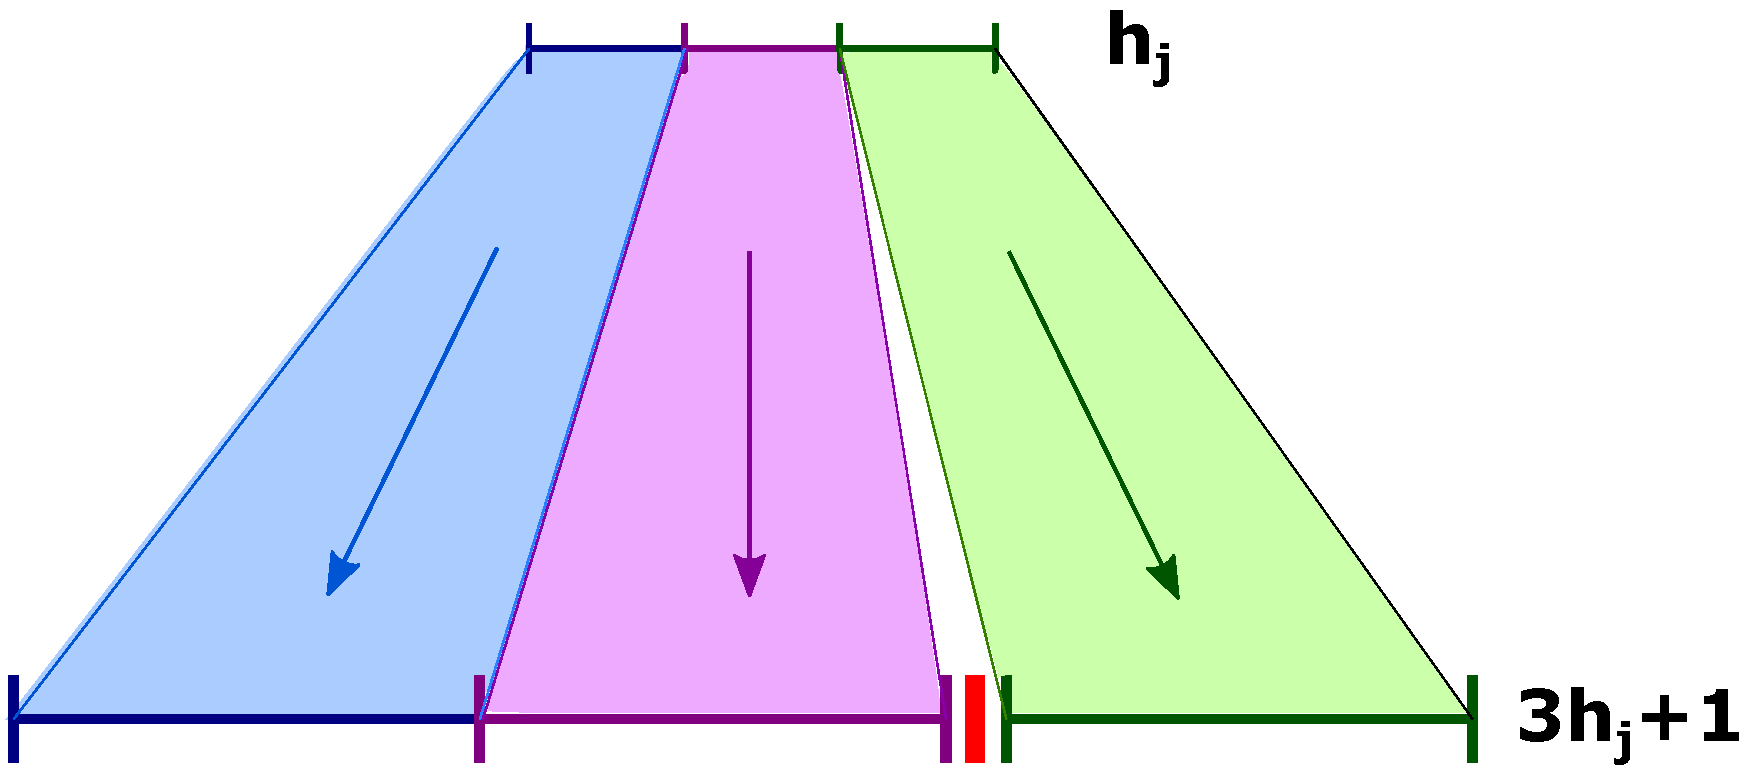
\includegraphics[height=35mm]{cutting-and-stacking.pdf}}\end{center}
    \begin{itemize}
    \item Сдвиг на группе $3$-адических чисел
    \end{itemize}
  \begin{flushright}
  
  \end{flushright}
\end{frame}

\begin{frame}
    \frametitle{Обобщённый автоморфизм Шакона}
    Определим аналогичный автоморфизм, заменив $3$ на произвольное $p \ge 3$:
    \begin{itemize}
    \item Подстановка $0 \to 00\ldots010, \quad 1 \to 1$
    \item Преобразование отрезков: $h_1 = 1,\ h_{j+1} = \mathbf{p}h_j + \pmb{\Delta_{p-2}}$\\
    $\Delta_{n} = \sum\limits_{k=0}^n k = \frac{n(n+1)}{2}$
    \item \textbf{Сдвиг на группе $\pmb{\Gamma}$}
    \end{itemize}

\end{frame}

\begin{frame}
    \frametitle{Группа $\Gamma$}
    $\Gamma := \left\{x = \left(x_0, x_1, x_2, \ldots \right), x_k \in \mathbb{Z}_p=\{0, 1, \ldots, p - 1\} \right\}$\\
    $\lambda$ --- мера Хаара на $\Gamma$. \\
    Определим сохраняющие меру $\lambda$ преобразования $\Gamma$:\\
    \begin{itemize}
    \item $\sigma:\ x=\left(x_0, x_1, x_2, \ldots \right) \mapsto \sigma x = \left(x_1, x_2, \ldots \right)$
    \item $S:\ x \mapsto x + 1$, где $1:=(1,0,0,\ldots)$
    \end{itemize}
    Определим функционал $\phi: \Gamma \setminus \{(p-1,p-1,\ldots)\} =: \Gamma' \rightarrow \mathbb{Z}$:\\
    \[\phi(x):=x_i\text{, если }x=(p-1, \ldots, p-1, x_i, x_{i+1}, \ldots)\]
    \[\phi^{(0)}(x):=0;\quad \phi^{(m)}(x):=\phi(x)+\phi(Sx)+\ldots+\phi(S^{m-1}x)\]
\end{frame}

\begin{frame}
    \frametitle{Обобщённый автоморфизм Шакона на группе $\Gamma$}  
    $X_n := \left\{(x, i): x \in \Gamma, 0 \le i \le h_n - 1 + \phi(x)\right\}$\\    
    \[
        T_n(x, i):= \begin{cases} 
            (x, i+1) & \text{, если } i+1 \le h_n-1+\phi(x)\\
            (Sx, 0) & \text{, если } i = h_n - 1 + \phi(x)
            \end{cases}
    \]
    \[\psi: X_n \rightarrow X_{n+1},\ \psi_n(x, i) := (\sigma x, x_0 h_n + i + \mathbb{I}_{x_0 = p-1})\]
  \begin{center}
  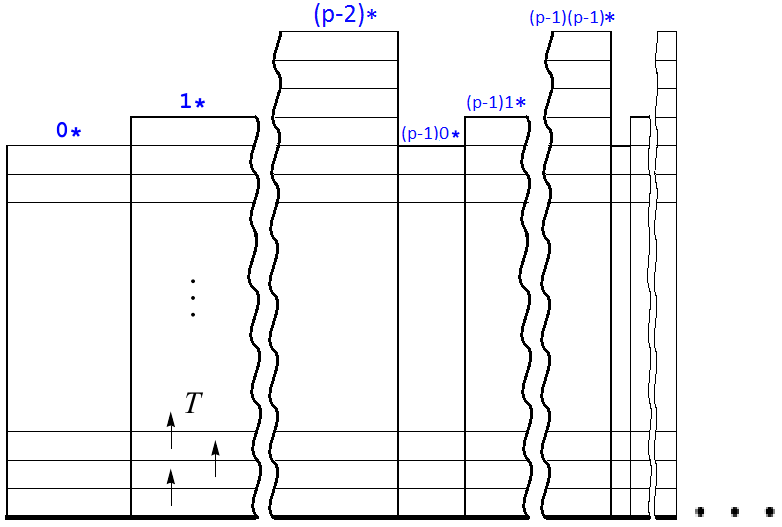
\includegraphics[height=35mm]{gen_stack.png}
  \end{center}
\end{frame}


\subsection{Характеристические полиномы}


\begin{frame}
    \frametitle{Построение полиномов}  
    \[\phi(x):=x_i\text{, если }x=(p-1, \ldots, p-1, x_i, x_{i+1}, \ldots)\]
    \[\phi^{(0)}(x):=0;\quad \phi^{(m)}(x):=\phi(x)+\phi(Sx)+\ldots+\phi(S^{m-1}x)\]
    Определим $\pi_m$ как функцию вероятности значений $\phi^{(m)}$:
    \[\pi_m(j) = \lambda(\phi^{(m)}=j), \quad j \in \mathbb{Z}\]
    Полиномы $P_m^p$ --- производящие функции последовательностей $\pi_m$:
    \[P_m^p(t):= \mathbb{E}_\lambda\left[ t^{\phi^{(m)}(x)}\right] = \sum\limits_{j=0}^m \pi_m(j) t^j \]
\end{frame}


\subsection{Известные результаты}


\begin{frame}
  \frametitle{Предельные теоремы}
  \textbf{E.Janvresse, T. de la Rue, A.Prikhodko., V.Ryzhikov, '13}
  
  \bigskip
  $T$ --- классическое преобразование Шакона ($p=3$).\\
  $\hat{T}$ --- оператор Купмана: $\hat{T}f(x) := f(Tx),\quad f \in L_2(\Gamma), x \in \Gamma$\\
  \bigskip
  {\bf Теорема 1.} $\Hat T^{mh_n} \wto P_m^3(\hat{T})$
  
  {\bf Теорема 2.}
  $$
    \mathcal{L} = \overline{\{\hat{T}^k \where k \in \Set{Z}\}} = \{P_{m_1}^3(\hat{T})\cdots P_{m_r}^3(\hat{T})\hat{T}^s,\ \Theta\},
  $$
  $\Theta$ --- ортогональный проектор на подпространство констант. \\

\end{frame}


\begin{frame}
  \frametitle{Предельные теоремы}
  \textbf{E.Janvresse, T. de la Rue, A.Prikhodko., V.Ryzhikov, '13}\\ \bigskip

  {\bf Теорема 3.}

    \[P_{3m}(t)=t^m P_m^3(t)\]
    \[P_{3m+1}(t)=\frac{1}{3} t^m \left((1+t)P_m^3(t) + P_{m+1}^3(t) \right)\]
    \[P_{3m+2}(t)=\frac{1}{3} t^m \left(tP_m^3(t) + (1+t)P_{m+1}^3(t) \right)\]
    
   Начальные условия: $P_0^3 = 1,\quad P_1^3 = \frac{1}{2}(1+t)$
\end{frame}


\begin{frame}
  \frametitle{Свойства полиномов}
  \begin{itemize}
   \item Коэффициенты симметричны
   \item Последовательности коэффициентов унимодальны
   \item Гипотеза: все корни вещественны
   \item Семейство $P_m^3$ содержит классы неприводимых полиномов над $\mathbb{Q}$
  \end{itemize}
 \end{frame}

\section{Палиндромическое свойство}
\subsection{Определения}
\begin{frame}
    \frametitle{Палиндромическое свойство}
    Напоминание: $\pi_m(j) = \lambda(\phi^{(m)}=j),\quad P_m^p(t):= \mathbb{E}_\lambda\left[ t^{\phi^{(m)}(x)}\right] = \sum\limits_{j=0}^m \pi_m(j) t^j$
    
    Пусть $\phi_\star = \min\limits_x \phi(x), \phi^\star = \max\limits_x \phi(x), \delta=\phi^\star - \phi_\star$.
    
     Палиндромическое свойство: $\forall j,\ 0 \le j \le m\delta:   \pi_m(m\phi_\star + j)=\pi_m(m\phi^\star-j)$
     \center{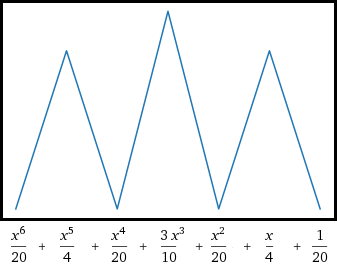
\includegraphics[scale=0.5]{palindromic}}
\end{frame}

\begin{frame}
    \frametitle{Обобщение $\phi$}

    $$
    \phi(x) = \begin{cases}
                    \omega(x_0), & 0 \le x_0 \le p - 2 \\
                    \phi(\sigma x), & x_0 = p - 1
                \end{cases}
    $$
    Автоморфизм Шакона: $\omega(j)=j$.\\

    Какие свойства $\omega$ достаточны для палиндромичности?
\end{frame}

\subsection{Теорема о палиндромичности}
\begin{frame}
\frametitle{Антипалиндромическое свойство}
Функцию $\omega$ назовём \textit{антипалиндромичной}, если
\[\begin{cases}
	\mathrm{Ran }\ \omega = \{0,1, \ldots, \zeta\} \\
	\forall j,\ 0 \le j \le p-2: \  \omega(j) + \omega(p-2-j) = \zeta
\end{cases}\]
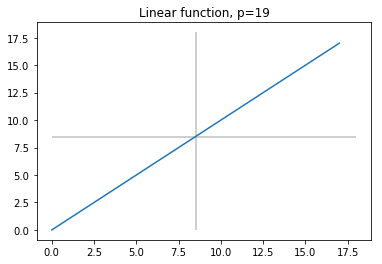
\includegraphics[width=0.5\linewidth]{linear}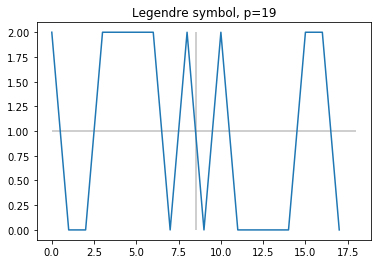
\includegraphics[width=0.5\linewidth]{legendre}
\end{frame}

\begin{frame}
\frametitle{Достаточное условие}
\textbf{Теорема.}
\begin{center}$\phi$ палиндромична $\iff$ $\omega$ антипалиндромична \end{center}
 
\textbf{Техническая лемма.}
Если $\omega$ антипалиндромична, то $$\{\phi(S^j x)\}_{j \ge 0} \overset{d}{=} \{ \zeta - \phi(S^{-j} x)\}_{j \ge 0}$$

\textbf{Лемма о наследовании.}
Если $\omega$ порождает палиндромичную $\phi$, это же верно для $a\omega+b$.
\end{frame}

\subsection{Пример}
\begin{frame}
\frametitle{Первые полиномы для p=3,4,5}
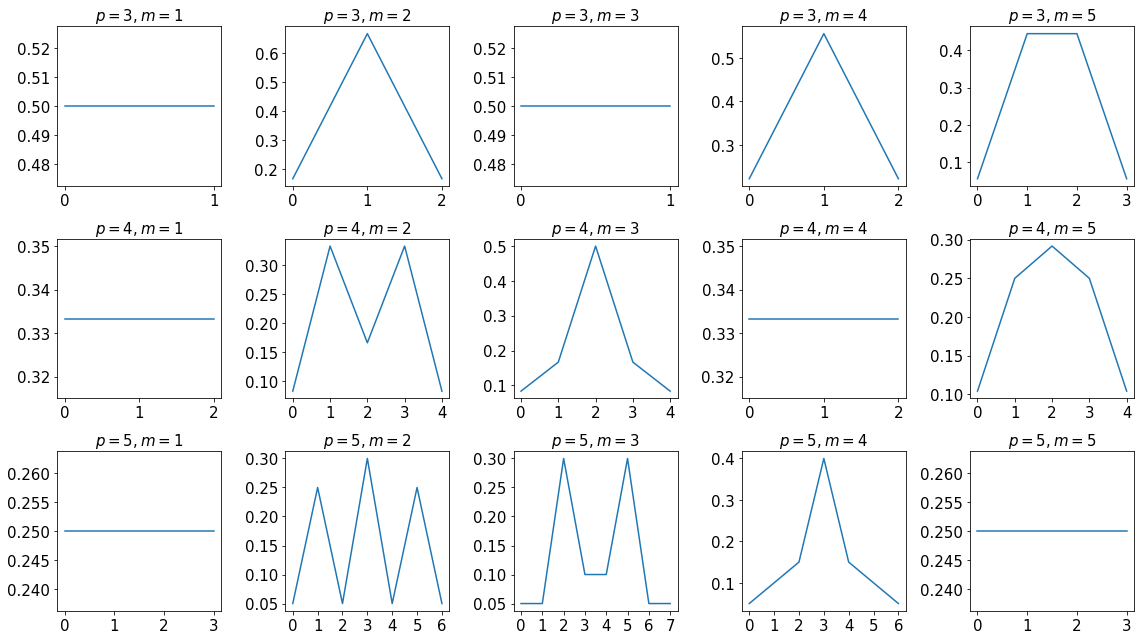
\includegraphics[width=\linewidth]{distributions_with_labels}
\end{frame}


\section{Рекуррентные соотношения}

\begin{frame}
    \frametitle{Результат для произвольного $p$}
     {\bf Theorem.}\\ \bigskip
     Пусть $p \ge 3,\ m \ge 0$, $1 \le k \le p-1$. Тогда
     \bigskip 
     \begin{eqnarray*} 
     P_{pm}^p(t) & = &  ~~t^{\Delta_{p-2} m}\ P_m^p(t)\ ; \\
     P_{pm+k}(t) & = &  ~~\frac{1}{p} t^{\Delta_{p-2} m + \Delta_{k-1}}\sum\limits_{j=0}^{p-k-1} t^{jk} P_m^p(t) + \\
     & & + \frac{1}{p} t^{\Delta_{p-2} m + \Delta_{k-2}}\sum\limits_{j=0}^{k-1} t^{j(p-k)} P_{m+1}^p(t) 
      \end{eqnarray*}
\end{frame}


\section{Степени полиномов}
\subsection{Предпосылки}

\begin{frame}
\frametitle{Степени. Определения}

$$P_m^p(t) = b_0 t^{d_m} + b_1 t^{d_{m}+1} + \ldots + b_{n}t^{D_m}$$
\begin{itemize}
\item$D_m^p = \max\limits_{x \in \Gamma'} \phi^{(m)}(x)$ --- верхняя степень
\item$d_m^p = \min\limits_{x \in \Gamma'} \phi^{(m)}(x)$ --- нижняя степень
\item$S_m = D_{m+1}^p - D_{m}^p$
\item$s_m = d_{m+1}^p - d_m^p$
\end{itemize}
\end{frame}


\begin{frame}
\frametitle{Рекуррентные соотношения для степеней}

\textbf{Верхняя степень}
\begin{align*}
  D_{pm}^p &= m \Delta_{p-2} + D_m^p \\
  D_{pm+k}^p &= m \Delta_{p-2}+(p-k)(k-1)+\Delta_{k-2}+D_m^p+\\
   &+ \mathrm{max}\{p-k-1, s_m\},
\end{align*}

\textbf{Нижняя степень}
\begin{align*}
  d_{pm}^p &= m \Delta_{p-2} + d_m^p \\
  d_{pm+k}^p &= m \Delta_{p-2}+d_m^p + \mathrm{min}\{k-1, d_{m+1}^p-d_m^p\}
\end{align*}
\end{frame}

\subsection{Степени и подстановки}
\begin{frame}
\frametitle{Структура $S_m$ и $s_m$}
$S_m = D_{m+1}^p-D_m^p, \quad s_m = d_{m+1}^p-d_m^p$.\bigskip\\

 $\{S_m\}_{m \ge 0}$ порождается подстановками:
\begin{itemize}
\item $S_0 = p-2$
\item $\forall j \in \left[0, \ldots, p-2 \right]: $\\$ j \mapsto (p-2, p-1,\ldots,j - 1, j, j , j+1, \ldots, 1, 0)$
\end{itemize}
\bigskip
 $\{s_m\}_{m \ge 0}$ порождается подстановками:
\begin{itemize}
\item $s_0 = 0$
\item $\forall j \in \left[0, \ldots, p-2 \right]: $\\$ j \mapsto (0, 1,\ldots,j - 1, j, j , j+1, \ldots, p-1, p-2)$
\end{itemize}
\end{frame}

\begin{frame}
\frametitle{Пример}
Пусть $p=5$. Вычислим первые члены $\{S_m\}$.\bigskip\\

\begin{itemize}
\item $3 \mapsto 33210$
\item $2 \mapsto 32210$
\item $1 \mapsto 32110$
\item $0 \mapsto 32100$
\end{itemize}

$3 \mapsto 33210 \mapsto 33210\ 33210\ 32210\ 32110\ 32100 \mapsto \ldots$
\end{frame}

\begin{frame}
\frametitle{Графики}
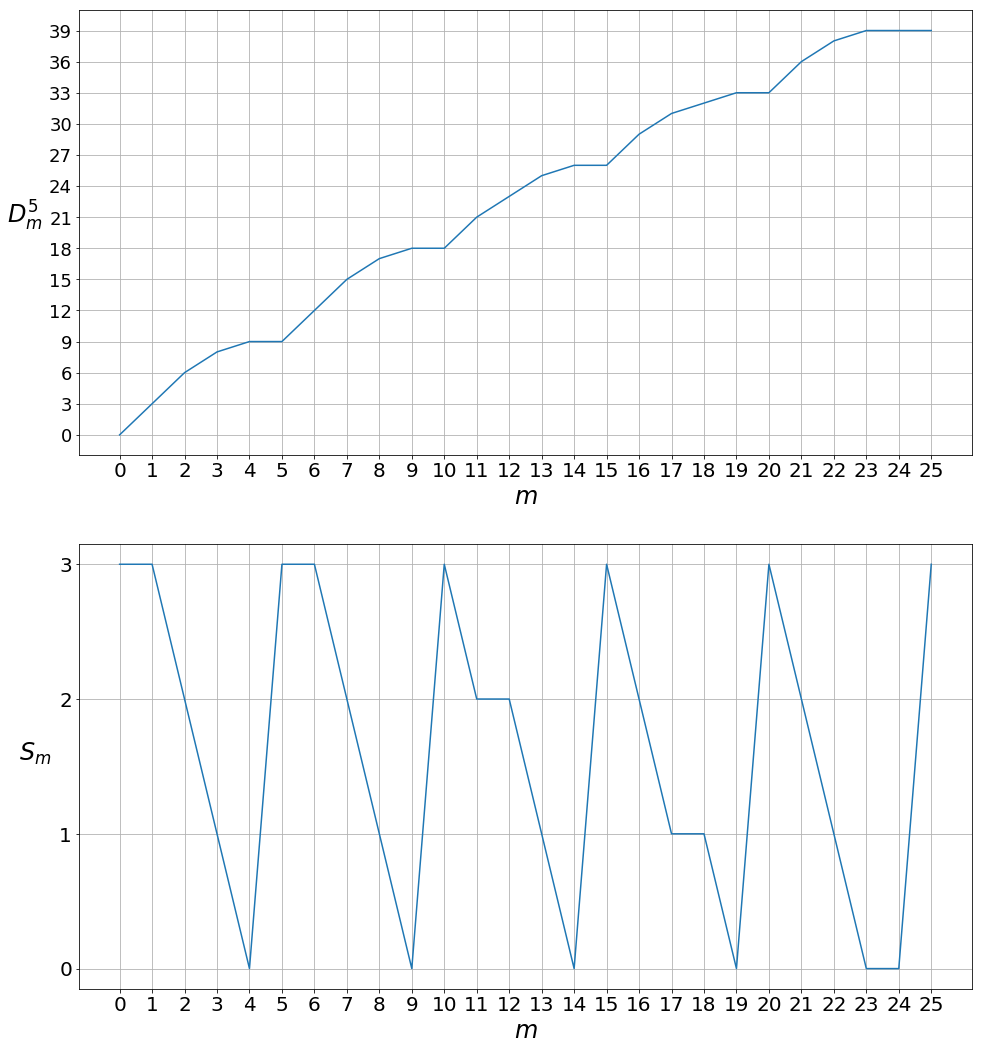
\includegraphics[width=0.5\linewidth]{degrees_big}
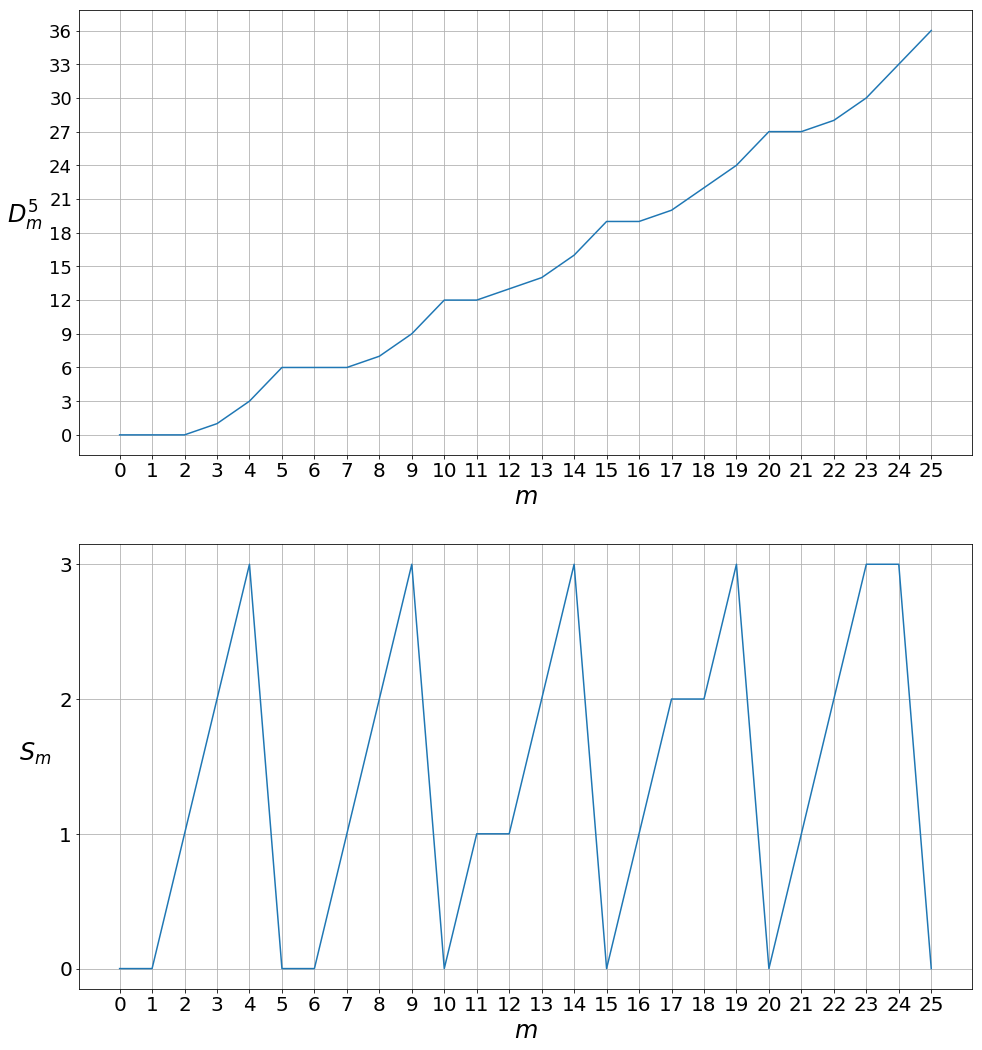
\includegraphics[width=0.5\linewidth]{degrees_small}
\end{frame}

\subsection{Симметризованные полиномы}
\begin{frame}
\frametitle{Определения}
$D_m$ --- параметр сдвига распределения $\pi_m$.\\
Как получить центрированное распределение?
\bigskip\\
\textbf{Центрированные полиномы}: $\bar{P}_m^p(t) = t^{-d_m}P_m^p(t)$
\begin{itemize}
\item $\bar{P}_m^p(t) = b_0 + b_1 t + \ldots + b_n t^n$
\item Нельзя описать $d_m$ алгебраически $\implies$ \\сложно вычислить!
\end{itemize}
\end{frame}

\begin{frame}
\frametitle{Симметризованная форма}
Замечательное свойство степеней: $S_m + s_m = p-2 = const$
Положим $\delta_m^p = \frac{1}{2}(D_m + d_m) = \frac{1}{2}(p-2)m$
\bigskip\\
\textbf{Симметризованные полиномы}: $\SymPol{p}{m}(t) = t^{-\delta_m}P_m^p(t)$
\begin{itemize}
\item $\SymPol{p}{m}(t) = b_{-\frac{n}{2}}t^{-\frac{n}{2}} + b_{-\frac{n}{2}+1} t^{-\frac{n}{2} + 1} + \ldots + b_{\frac{n}{2}-1} t^{\frac{n}{2} - 1} + b_{\frac{n}{2}}t^{\frac{n}{2}}$
\item Простая формула для $\delta_m^p \implies$\\
явные рекуррентные уравнения
\end{itemize}
\end{frame}

\begin{frame}
\frametitle{Рекуррентные соотношения}
\begin{align*}
    \SymPol{p}{pm}(t)&=\SymPol{p}{m}(t)\\
    \SymPol{p}{pm+k}(t)&=\frac{1}{p}\left(\sum\limits_{j=-\frac{p-k-1}{2}}^{\frac{p-k-1}{2}} t^{jk}\right)\SymPol{p}{m}(t)+\frac{1}{p}\left(\sum\limits_{j=-\frac{k-1}{2}}^\frac{k-1}{2} t^{j(p-k)}\right)\SymPol{p}{m+1}(t)
\end{align*}
\end{frame}

\section*{Заключение}
\begin{frame}
\frametitle{Вопросы для дальнейшего изучения}
\begin{itemize}
\item Слабое замыкание для обобщённого преобразования
\item Алгебраические свойства полиномов
\begin{itemize}
\item Неприводимость
\item Свойства корней
\end{itemize}
\end{itemize}
\end{frame}